\chapter{Θεωρητικό Υπόβαθρο}

%Το \en{Lorem Ipsum} είναι απλά ένα κείμενο χωρίς νόημα για τους επαγγελματίες της τυπογραφίας και στοιχειοθεσίας \cite{LoremIpsumAll}. Το \en{Lorem Ipsum} είναι το επαγγελματικό πρότυπο όσον αφορά το κείμενο χωρίς νόημα, από τον 15ο αιώνα, όταν ένας ανώνυμος τυπογράφος πήρε ένα δοκίμιο και ανακάτεψε τις λέξεις για να δημιουργήσει ένα δείγμα βιβλίου. Όχι μόνο επιβίωσε πέντε αιώνες, αλλά κυριάρχησε στην ηλεκτρονική στοιχειοθεσία, παραμένοντας με κάθε τρόπο αναλλοίωτο. Έγινε δημοφιλές τη δεκαετία του '60 με την έκδοση των δειγμάτων της \en{Letraset} όπου περιελάμβαναν αποσπάσματα του \en{Lorem Ipsum}, και πιο πρόσφατα με το λογισμικό ηλεκτρονικής σελιδοποίησης όπως το \en{Aldus PageMaker} που περιείχαν εκδοχές του \en{Lorem Ipsum}.
\section{Τεχνολογίες του \en{software development}}

\subsection{\en{Django Framework},\en{Paramiko}, \en{Netmiko} και \en{Napalm}}

Το \en{Django} είναι ένα \en{backedn framework} το οποίο βασίζεται στη γλώσσα προγραμματισμού \en{Python}. Με το \en{Django}, μπορείτε να μεταφέρετε τις εφαρμογές Ιστού από την ιδέα στην κυκλοφορία μέσα σε λίγες ώρες. 
Το \en{Django} βοηθάει στο να στηθεί γρήγορα μία εφαρμογή ανάπτυξης ιστού έτσι ώστε να μπορούμε να εστιάσουμε στη σύνταξη της εφαρμογής και της λειτουργικότητάς της χωρίς να χρειάζεται να ανακαλύψουμε ξανά τον τροχό.
Είναι δωρεάν και ανοιχτού κώδικα. Ορισμένες από τις πιο μεγάλες εταιρίες στον πλανήτη χρησιμοποιούν την ικανότητα του
να κλιμακώνεται γρήγορα και με ευελιξία για να ανταποκρίνεται στις μεγαλύτερες απαιτήσεις κίνησης. Στη δικιά μας περίπτωση χρησιμοποιήθηκε το συγκεκριμένου
{Framework} γιατί θα μας έδινε τη δυνατότητα να φτιάξουμε μία εφαρμογή με μεγάλη επεκτασιμότητα και παράλληλα να μπορέσουμε να ενσωματώσουμε μεσα διαφορετικές τεχνολογίες.

Παράλληλα με το \en{Django} χρησιμοποιήθηκαν έτοιμες βιβλιοθήκες της \en{Python} προκειμένου να μπορέσουν να εκτελεστούν βασικές λειτουργίες της εφαρμογής όπως 
τα πρωτοκολλα επικοινωνίας. Θεωρούμε ότι η δημιουργία τέτοιων βιβλιοθηκών ξεφεύγει από τα όρια μιας διπλωματικής εργασίας καθώς απαιτεί πολύ χρόνο και ερευνητική
ενασχόληση που μόνο στα πλαίσια ενός διδακτορικού θα μπορούσε να υλοποιηθεί μιά τέτοια ιδέα. Παρακάτων παρουσιάζονται οι βιβλιοθήκες που χρησιμοποιήθηκαν και κάποια βασικά χαρακτηριστικά τους.

\subsection{\en{Paramiko}}
Το \en{Paramiko} είναι μια διασύνδεση καθαρά \en{Python} που υλοποιεί το πρωτόκολλο \en{SSH} έκδοσης 2 σε \en{Python}, παρέχοντας λειτουργικότητα τόσο πελάτη όσο και διακομιστή.
Το \en{Paramiko} μπορεί να επιτύχει υψηλές επιδόσεις σε χαμηλού επιπέδου κρυπτογραφικές έννοιες.
Οποιαδήποτε συσκευή που μπορεί να ρυθμιστεί μέσω \en{SSH} μπορεί επίσης να ρυθμιστεί από την \en{Python} με σενάρια με τη χρήση αυτής της μονάδας.

\subsection{\en{Netmiko}}
Το \en{Netmiko} είναι μια βιβλιοθήκη ανοικτού κώδικα για πολλούς προμηθευτές, που σημαίνει ότι πολλές συσκευές μπορούν να ρυθμιστούν από την \en{python}
χρησιμοποιώντας το \en{Netmiko}.
Ορισμένες από τις συσκευές που υποστηρίζει το \en{Netmiko} είναι οι εξής: \en{Cisco IOS}, \en{Juniper}, \en{Arista}, \en{HP} και \en{Linux}. 
Μπορεί επίσης να υποστηρίζει και άλλους προμηθευτές όπως η \en{Alcatel}, η \en{Huawei} και η \en{Ubiquity} αλλά περιορισμένα 
δοκιμές έχουν γίνει με αυτούς τους προμηθευτές.
Το \en{Netmiko} τρέχει πάνω από το \en{Paramiko} για να κάνει τη σύνδεση \en{SSH} σε συσκευές δικτύου λιγότερο περίπλοκη, πιο ευέλικτη και πιο εύκολη στη χρήση. Παρόλο που το \en{Netmiko} είναι ευκολότερο στη χρήση, όπως αναφέρθηκε 
παραπάνω, υποστηρίζει συγκεκριμένους προμηθευτές και μόνο έναν αριθμό συσκευών τους. Από την άλλη πλευρά,
το \en{Paramiko} μπορεί να χρησιμοποιηθεί για την επικοινωνία με οποιαδήποτε συσκευή που υποστηρίζει \en
{SSH}.
Τόσο το \en{Paramiko}όσο και το \en{Netmiko} αποτελούν εναλλακτικές επιλογές για συσκευές που δεν υποστηρίζουν 
\en{APIs}.

\subsection{\en{Napalm}}
Το \en{NAPALM} (\en{Network Automation and Programmability Abstraction Layer with Multivendor support}) είναι μια βιβλιοθήκη \en{Python} που υλοποιεί ένα σύνολο λειτουργιών για την αλληλεπίδραση με διαφορετικά λειτουργικά συστήματα συσκευών δικτύου χρησιμοποιώντας ένα ενοποιημένο \en{API}.
Το \en{NAPALM} υποστηρίζει διάφορες μεθόδους σύνδεσης με τις συσκευές, χειρισμού των ρυθμίσεων ή ανάκτησης δεδομένων. Το \en{Napalm} συνεπώς είναι μια βιβλιοθήκη \en{Python} που παρέχει ένα \en{API}
\en{(Application Programming Interface)} για την εργασία με συσκευές δικτύου. Έχει σχεδιαστεί για να απλοποιεί την
αυτοματοποίηση και τη διαχείριση του δικτύου με την αφαίρεση των υποκείμενων λεπτομερειών που σχετίζονται με τον εκάστοτε προμηθευτή και την παροχή μιας συνεπούς διεπαφής σε διαφορετικά δίκτυα. 
συσκευών.
Το \en{Napalm} επιτρέπει στους μηχανικούς και τους διαχειριστές δικτύων να αυτοματοποιούν κοινές εργασίες διαχείρισης δικτύου, όπως η διαμόρφωση, η παροχή, η παρακολούθηση και η 
αντιμετώπιση προβλημάτων. Υποστηρίζει πολλούς προμηθευτές συσκευών δικτύου, συμπεριλαμβανομένων των \en{Cisco}, \en{Juniper}, \en{Arista} και \en{Huawei}.
Το \en{Napalm} παρέχει ένα σύνολο κοινών λειτουργιών που μπορούν να εκτελεστούν σε συσκευές δικτύου, όπως η ανάκτηση πληροφοριών διαμόρφωσης, η εφαρμογή διαμόρφωσης 
αλλαγών, έλεγχος στατιστικών στοιχείων διασύνδεσης και συλλογή πληροφοριών τοπολογίας δικτύου παρέχει επίσης χαρακτηριστικά όπως υποστήριξη επαναφοράς, επικύρωση διαμόρφωσης 
αλλαγών διαμόρφωσης, και σύγκριση των διαφορών διαμόρφωσης μεταξύ συσκευών.
14
Το \en{Napalm} μπορεί να συνδυαστεί με βιβλιοθήκες \en{Python} όπως οι \en{Netmiko}, \en{Paramiko} και \en{Ansible} για τη δημιουργία σύνθετων ροών εργασίας αυτοματισμού δικτύου. Μπορεί επίσης να ενσωματωθεί 
με δημοφιλή εργαλεία παρακολούθησης δικτύου, όπως το \en{Prometheus} και το \en{Grafana}, για την παρακολούθηση της απόδοσης του δικτύου σε πραγματικό χρόνο.


\subsection{\en{Version Control} με \en{Git} και \en{GitHub} }

Το \en{Git} είναι ένα σύγχρονο σύστημα ελέγχου εκδόσεων (γνωστό και ως σύστημα διαχείρισης αναθεωρήσεων ή πηγαίου κώδικα), 
σχεδιασμένο με έμφαση στην ταχύτητα, την ακεραιότητα των δεδομένων και την υποστήριξη κατανεμημένων, μη γραμμικών ροών εργασίας. 
Στην παρούσα διπλωματική εργασία, θα αξιοποιήσουμε το \en{Git} για να διασφαλίσουμε την ορθή διαχείριση των εκδόσεων του λογισμικού, 
τόσο κατά τη διάρκεια της ανάπτυξης όσο και για την πιθανή μελλοντική χρήση και εξέλιξη της δουλειάς μας. Το \en{GIT} συνεπώς είναι απαραίτητο σε κάθε σοβαρό 
έργο ανάπτυξης, και αυτό δεν αποτελεί εξαίρεση. Παρέχει γρήγορη ανάπτυξη κώδικα, έκδοση και επιτρέπει διακλαδώσεις. Έχοντας το εγκατεστημένο στον 
τοπικό υπολογιστή ανάπτυξης και στο περιβάλλον παραγωγής επιτρέπει την εύκολη και γρήγορη ανάπτυξη στο περιβάλλον παραγωγής.
τον ήδη δοκιμασμένο κώδικα στο τοπικό περιβάλλον ανάπτυξης. Η έκδοση παρέχει τη δυνατότητα επαναφοράς σε προηγούμενες εκδόσεις κώδικα σε
περίπτωση που κάποιο άγνωστο σφάλμα εμφανιστεί σε μια νεότερη έκδοση. 

\subsection{Συνεχής Ενσωμάτωση και Παράδοση (\en{CI/CD}) }

Μόλις η εφαρμογή ιστού συνδεθεί με το απομακρυσμένο αποθετήριο, η τελευταία τάση στο
στον κόσμο του \en{DevOps} είναι η υλοποίηση ενός αγωγού \en{CI/CD}, ο οποίος ουσιαστικά
είναι μια αυτοματοποιημένη διαδικασία που ενεργοποιείται όταν νέος κώδικας δημοσιεύεται στο
απομακρυσμένο αποθετήριο. Αυτή η διαδικασία ξεκινάει τη δημιουργία κώδικα, εκτελεί κάποιες δοκιμές και
τέλος, αν όλα είναι εντάξει, αναπτύσσει αυτόματα τον κώδικα στην παραγωγή
περιβάλλον. Με αυτόν τον τρόπο, οι προγραμματιστές μπορούν να διασφαλίσουν ότι τίποτα δεν θα χαλάσει
στην παραγωγή και οι νέες λειτουργικότητες εξυπηρετούνται το συντομότερο δυνατό στους
πελάτη. Στην περίπτωσής μας τόσο η διπλωματική εργασία(\en{latex}) όσο και η εφαρμογή υλοποιήθηκαν με αυτή τη λογική.


\section{Τεχνολογίες του \en{Software deployment}}

\subsection{\en{Containers} και \en{Docker}}

Το \en{Docker} είναι μια πλατφόρμα που επιτρέπει τη δημιουργία, τη διανομή και την εκτέλεση εφαρμογών μέσα σε ελαφριά, απομονωμένα "κοντέινερ" (\en{containers}). 
Τα κοντέινερ περιλαμβάνουν ό,τι χρειάζεται μια εφαρμογή για να τρέξει, όπως κώδικα, βιβλιοθήκες και εξαρτήσεις, διασφαλίζοντας ότι θα λειτουργεί ομοιόμορφα 
ανεξάρτητα από το περιβάλλον στο οποίο εκτελείται. Με αυτόν τον τρόπο διευκολύνει τη διαχείριση και τη μεταφορά εφαρμογών από τον έναν υπολογιστή ή διακομιστή 
στον άλλον.

\subsection{\en{Kubernetes} και \en{Container Orchestration}}
Ο κυβερνήτης είναι ο διαχειριστής των με απλά λόγια ο διαχειριστής των \en{containers}. Είναι μια 
πλατφόρμα ανοικτού κώδικα για τη διαχείριση φορτίων εργασίας και υπηρεσιών που περιέχουν \en{containers}
, η οποία διευκολύνει τόσο τη δηλωτική διαμόρφωση όσο και την αυτοματοποίηση. 
Διαθέτει ένα μεγάλο, ταχέως αναπτυσσόμενο οικοσύστημα. Οι υπηρεσίες, η υποστήριξη και τα εργαλεία του \en{Kubernetes} είναι ευρέως διαθέσιμα.

\section{Αυτοματοποίηση Διαχείρισης Δικτύου}

\subsection{\en{Network Automation}}

Η αυτοματοποίηση δικτύου δεν περιορίζεται μόνο στη διαμόρφωση συσκευών. 
Αντιθέτως, το πιο σημαντικό μέρος της αυτοματοποίησης δικτύου, που συμβάλλει στη μείωση των ανθρώπινων σφαλμάτων, 
είναι η δυνατότητα που παρέχει στους διαχειριστές να αυτοματοποιούν διαδικασίες για τη διενέργεια ελέγχων συμμόρφωσης και 
επικύρωσης της τρέχουσας διαμόρφωσης ή οποιασδήποτε διαμόρφωσης πρόκειται να εφαρμοστεί.

Αυτό έχει ως αποτέλεσμα τη μείωση του χρόνου υλοποίησης των αλλαγών στο δίκτυο και του κινδύνου διακοπής ή διατάραξης της υπηρεσίας, 
ενώ ελαχιστοποιεί την πιθανότητα ανθρώπινου λάθους και διασφαλίζει την ευθυγράμμιση με τις πολιτικές του δικτύου.Μία ακόμη διαδικασία που μπορεί να 
αυτοματοποιηθεί είναι η επίλυση προβλημάτων. Όταν προκύπτει κάποιο πρόβλημα στο δίκτυο, το πρώτο βήμα για την αντιμετώπισή του είναι η συλλογή πληροφοριών. 
Η συλλογή πληροφοριών από κάθε συσκευή μπορεί να είναι χρονοβόρα και περίπλοκη, κάτι που είναι κρίσιμο, διότι συνήθως, στο μεταξύ, το δίκτυο ή ένα μέρος του παραμένει 
εκτός λειτουργίας.

Με τη χρήση της αυτοματοποίησης δικτύου, μπορούμε να αυτοματοποιήσουμε τις εντολές που απαιτούνται για τη 
συλλογή των απαραίτητων πληροφοριών για την επίλυση προβλημάτων και να έχουμε πρόσβαση σε αυτές σε πραγματικό χρόνο.
Η προγραμματική συλλογή αυτών των πληροφοριών επιτρέπει και τον έλεγχο τους σε πραγματικό χρόνο. Ο έλεγχος πληροφοριών σε πραγματικό χρόνο και η λήψη αποφάσεων για τις απαραίτητες ενέργειες, εάν, για παράδειγμα, αλλάξει η τιμή κάποιου παραμέτρου, όπως το MTU, αποτελεί μία τρίτη πτυχή της αυτοματοποίησης δικτύου, γνωστή ως αυτοματοποιημένη παρακολούθηση. Η αυτοματοποιημένη παρακολούθηση βοηθά στην πρόληψη βλαβών που προκαλούνται από αποτυχίες υλικού.



\subsection{\en{Cisco IOS}}
Το \en{IOU} σημαίνει \en{IOS on Unix} είναι μια εικονική έκδοση του λογισμικού \en{IOS} της \en{Cisco} που 
μπορεί να χρησιμοποιηθεί για σκοπούς προσομοίωσης και δοκιμής δικτύου. Επιτρέπει στους μηχανικούς δικτύου να δημιουργούν εικονικές τοπολογίες δικτύου και να εξασκούνται σε διάφορες εργασίες δικτύου, 
όπως η διαμόρφωση δρομολογητών και μεταγωγέων, χωρίς να απαιτείται φυσικό υλικό. Το πλεονέκτημα του \en{GNS3} σε σχέση με εφαρμογές άλλες όπως το \en{Packet tracer} είναι ότι το \en{GNS3} 
μπορεί να σηκώσει πραγματικά \en{images} άρα πραγματικό λογισμικό συνεπώς οι λειτουργίες που μπορείς να κάνεις είναι πολύ περισσότερες.


\subsection{\en{REST APIs} για Δικτυακές Συσκευές \en{Cisco}}
Το \en{Django}, σε συνδυασμό με το \en{Django REST Framework (DRF)}, είναι μια ισχυρή επιλογή για την κατασκευή \en{backend} 
εφαρμογών που αλληλεπιδρούν με \en{REST APIs}, συμπεριλαμβανομένων των \en{APIs} της \en{Cisco}. Μπορείς να χρησιμοποιήσεις το \en{Django} 
για να αυτοματοποιήσεις και να διαχειριστείς δικτυακές συσκευές της \en{Cisco} μέσω αυτών των \en{APIs}.


\subsection{\en{GNS3} και Εικονικά Δίκτυα}

Το \en{GNS3} Είναι ένα εργαλείο προσομοίωσης δικτύων ανοικτού κώδικα που επιτρέπει στους χρήστες να προσομοιώσουν 
σύνθετες τοπολογίες δικτύων στους υπολογιστές τους. Μηχανικοί δικτύων και φοιτητές 
το χρησιμοποιούν ευρέως για να μάθουν και να εξασκηθούν σε έννοιες δικτύωσης, να δοκιμάσουν διαμορφώσεις δικτύου και να δημιουργήσουν εικονικά περιβάλλοντα δικτύου.


Το \en{GNS3} υποστηρίζει διάφορες συσκευές δικτύου, όπως δρομολογητές, μεταγωγείς και τείχη προστασίας 
από διάφορους προμηθευτές, συμπεριλαμβανομένων των \en{Cisco}, \en{Juniper}, \en{Nokia} και άλλων. Επιτρέπει στους χρήστες να 
προσομοιώσουν διάφορα σενάρια και διαμορφώσεις δικτύου και να δοκιμάσουν τη συμπεριφορά των 
συσκευών δικτύου σε ένα ελεγχόμενο περιβάλλον. 

Στην επιστήμη της πληροφορικής, η εικονικοποίηση \en{virtualization} είναι ένας ευρύς όρος 
των υπολογιστικών συστημάτων που αναφέρεται σε έναν μηχανισμό αφαίρεσης, 
στοχευμένο στην απόκρυψη λεπτομερειών της υλοποίησης και της κατάστασης
ορισμένων υπολογιστικών πόρων από πελάτες των πόρων αυτών 
(π.χ. εφαρμογές, άλλα συστήματα, χρήστες κλπ). 
Η εν λόγω αφαίρεση μπορεί είτε να αναγκάζει έναν πόρο να 
συμπεριφέρεται ως πλειάδα πόρων (π.χ. μία συσκευή αποθήκευσης σε διακομιστή τοπικού δικτύου),
είτε πολλαπλούς πόρους να συμπεριφέρονται ως ένας (π.χ. συσκευές αποθήκευσης σε κατανεμημένα συστήματα). 

Η εικονικοποίηση δημιουργεί μία εξωτερική διασύνδεση η οποία αποκρύπτει την 
υποκείμενη υλοποίηση (π.χ. πολυπλέκοντας την πρόσβαση από διαφορετικούς χρήστες).
Αυτή η προσέγγιση στην εικονικοποίηση αναφέρεται ως εικονικοποίηση πόρων. 
Μία άλλη προσέγγιση, ίδιας όμως νοοτροπίας, είναι η εικονικοποίηση πλατφόρμας,
όπου η αφαίρεση που επιτελείται προσομοιώνει ολόκληρους υπολογιστές. Το αντίθετο της εικονικοποίησης είναι η διαφάνεια: 
ένας εικονικός πόρος είναι ορατός, αντιληπτός, αλλά στην πραγματικότητα ανύπαρκτος, 
ενώ ένας διαφανής πόρος είναι υπαρκτός αλλά αόρατος. 
 
Θα εξηγήσουμε την εικονικοποίηση στην δικιά μας περίπτωση. Το πρώτο επίπεδο είναι αυτό του υλικού. Η εικονικοποίηση
σα τεχνολογία εικονοποιεί το υλικό για να μπορέσει να δώσε πόρους στις εικονικές μηχανές. Η υλοιποίηση
της εικονικοποίησης γίνεται με λογισμικό \en{hypervisor}. Στη δικιά μας περίπτωση ο \en{hypervisor} είναι 
το \en{Virtual Box} ο οποίος είναι ένας τύπου Β \en{hypervisor}. Ο \en{hypervisor} τύπου 2 είναι μια εφαρμογή εγκατεστημένη 
στο λειτουργικό σύστημα του κεντρικού υπολογιστή το οποίο μας δίνει τη δυνατότητα να σηκώσουμε 
εικονικές μηχανές άλλων λειτουργικών συστημάτων πάνω στο ήδη υπάρχον σύστημα.

Οι παρακάτω εικόνες μπορούν να εξηγήσουν σχηματικά τη γενική καθώς και την ειδική αρχιτεκτονική.

\begin{figure}[htb]
	\centering
	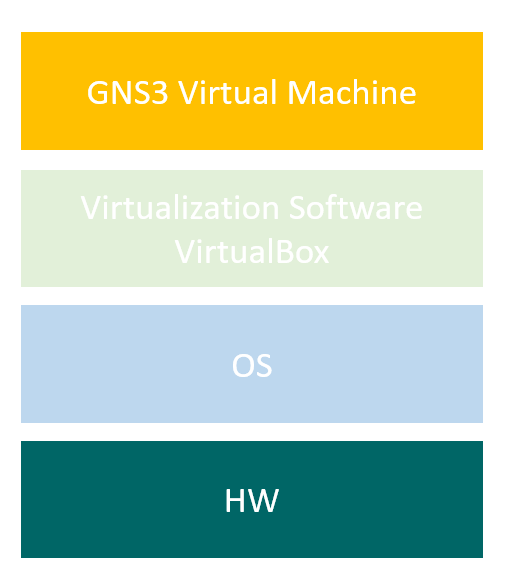
\includegraphics[width=0.5\textwidth]{graphics/Architecture_virtualbox.PNG}
	\caption{\en{Virtualization} Γενική αρχιτεκτονική}
\end{figure}

\begin{figure}[htb]
	\centering
	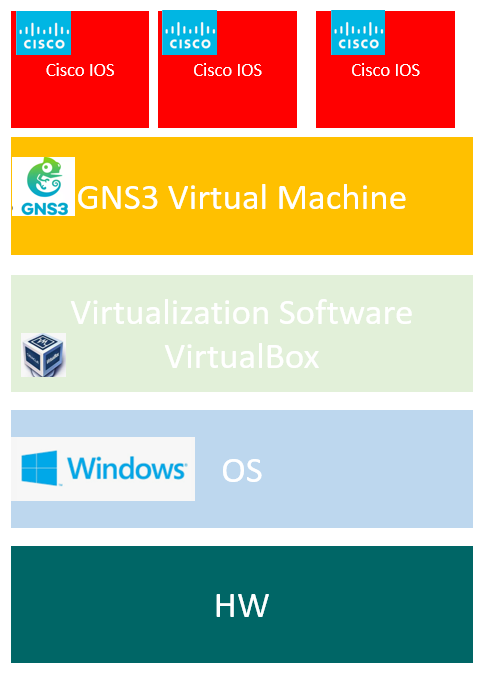
\includegraphics[width=0.5\textwidth]{graphics/virtualization_architecture.PNG}
	\caption{\en{Virtualization} Γενική αρχιτεκτονική}
\end{figure}

\section{Πρόγραμμα εικονοποίσης για το \en{GNS3 VM-VirtualBox}}

Το \en{Oracle VM VirtualBox} ή \en{VirtualBox} (πρώην \en{Sun VirtualBox}, \en{Sun xVM VirtualBox} και \en{Innotek VirtualBox}) είναι υπερεπόπτης
ανοιχτού κώδικα για υπολογιστές \en{x86} που αναπτύσσεται από την \en{Oracle Corporation}.
Αναπτύχθηκε αρχικά από την \en{Innotek GmbH}
και αποκτήθηκε από τη \en{Sun Microsystems} το 2008, η οποία εξαγοράστηκε από την \en{Oracle} το 2010.

Το \en{VirtualBox} μπορεί να εγκατασταθεί σε διάφορα λειτουργικά συστήματα, συμπεριλαμβανόμενων των \en{Linux, macOS, Windows, Solaris} και \en{OpenSolaris}.
Υπάρχουν επίσης μεταφορές για το \en{FreeBSD} και το \en{Genode}.
Υποστηρίζει τη δημιουργία και τη διαχείριση εικονικών μηχανών που εκτελούν εκδόσεις και παραλλαγές των \en{Microsoft Windows, Linux, BSD, Solaris, Haiku, OSx86}
και άλλα, καθώς και περιορισμένη εικονικοποίηση \en{macOS}.
Για ορισμένα λειτουργικά συστήματα είναι διαθέσιμο ένα πακέτο \en{"Guest Additions"} από μηχανές συσκευών και εφαρμογές συστήματος
που συνήθως βελτιώνει την απόδοση, ειδικά των γραφικών, επίσης δίνει την δηνατότητα στον χρήστη να μεταφέρει αρχεία ή κείμενο από μία εικονική μηχανή στον υπολογιστή του χρήστη και να αυξήσει την ανάλυση του παράθυρου της μηχανή. 
Στην εικόνα 3.4 μπορούμε να δούμε το \en{VirtualBox} και την εικονική μηχανή \en{GNS3 VM}

\begin{figure}[htb]
	\centering
	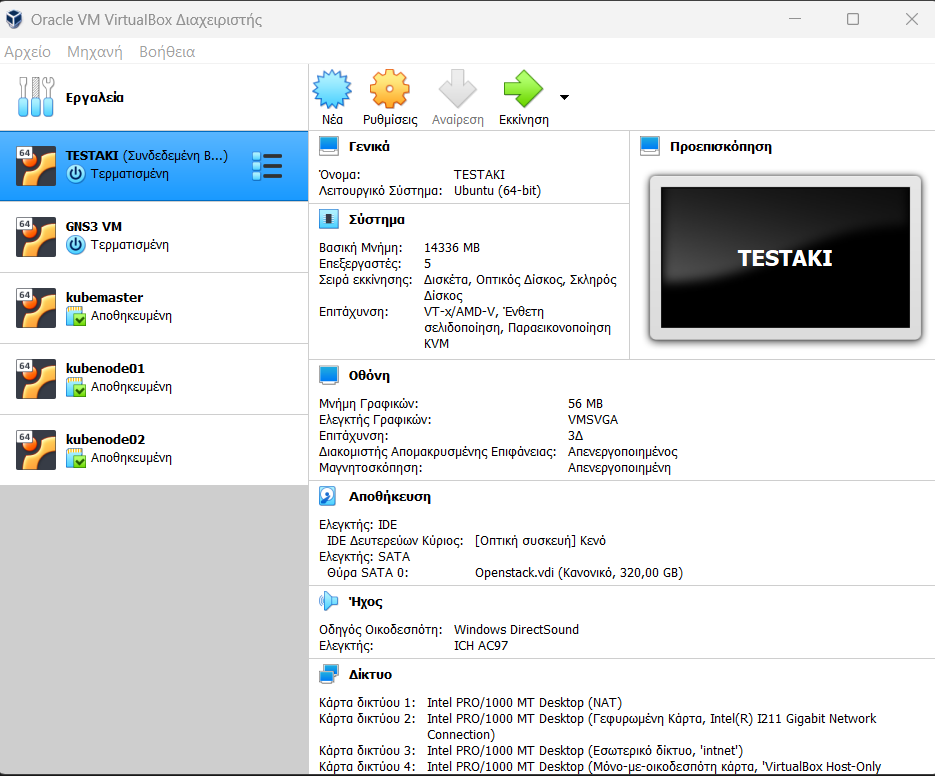
\includegraphics[width=0.9\textwidth]{graphics/virtualbox.PNG}
	\caption{\en{Virtualbox} }
\end{figure}


%\begin{equation}
%	y = \alpha x + \beta
%\end{equation}

%Αντίθετα με αυτό που θεωρεί η πλειοψηφία, το \en{Lorem Ipsum} δεν είναι απλά ένα τυχαίο κείμενο. Οι ρίζες του βρίσκονται σε ένα κείμενο Λατινικής λογοτεχνίας του 45 π.Χ., φτάνοντας την ηλικία του πάνω από 2000 έτη.


%\begin{figure}[htb]
%	\centering
%	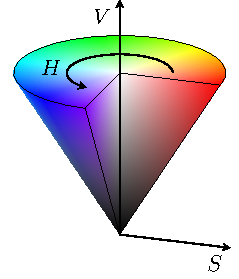
\includegraphics{tikz/hsv_cone/hsv_cone.pdf}
%	\caption{Ο χρωματικός χώρος \en{HSV}.}
%\end{figure}
